\section{Photon Detector Simulation}
\label{sec:dp-pds-simulation}

A detailed simulation of the \dword{pds} response is essential both to compare with data from \dword{pds} prototypes (see Section~\ref{sec:dp-pds-prototypes}) and to validate the \dword{fd} baseline design for its projected performance (see Section~\ref{sec:dp-pds-performance}).

%%%%%%%%%%%%%%%%%%%%%%%%%%%%%%%%%%%%%%%%%%%%%%%%%%%%%%%%%%%%%%%%%%%

\subsection{Simulation Framework And Assumptions}
\label{subsec:dp-pds-simulation_assumptions}

The simulation of the \dword{pds} response is integrated in \dword{larsoft}, the liquid argon software toolkit used by the \dune collaboration for simulation and reconstruction. The simulation is divided in three steps: light generation, light propagation, and light detection.

%For a \dword{mip}, an energy of about \SI{2}{\MeV/\cm} is deposited in \dword{lar}. 
A \dword{mip} deposits an energy of about \SI{2}{\MeV/\cm} in \dword{lar}. Through decays of excited argon states and ion recombination, about \num{40000} scintillation photons are emitted per \si{\MeV} deposited at null drift field. At the nominal drift field of \SI{500}{\V/\cm}, this amount reduces down to about \num{24000} photons per \si{\MeV} as the recombination process weakens. This signal, known as S1 (see Section~\ref{sec:dp-pds-overview}), is common to the \dword{sp} and \dword{dp} technologies.

In the gas layer of the \dword{dp} design, the electrons are amplified through a Townsend avalanche process in the \dword{lem} holes and %lead to 
yield an electroluminescence signal called S2 (see Section~\ref{sec:dp-pds-overview}). The electroluminescence gain, $G_{EL}$, i.e., the number of photons produced per electron crossing the liquid-gas interface, depends on the voltages applied to the \dword{lem}. In our simulations, we typically assume a gain of \SI{300}{photons per extracted electron}. The S1 and S2 signals have similar characteristics for wavelength and time constant. %s. 

%Because of different mechanisms during photon propagation (Rayleigh scattering, absorption by impurities in the \lar or by elements constituting the detector), only \num{1e-3} fraction of the 
Because of the Rayleigh scattering and absorption (by impurities in the \lar or by detector elements) that take place during photon propagation, a fraction of only \num{1e-3}  of the photons produced in the \lar active volume reaches the \dword{pmt} photocathodes. Directly simulating the large number of photons generated for each track crossing the active volume would require a considerable amount of CPU power and time. %Profiting from the fact that 
Instead, since the photon emission is isotropic and the detector is uniform and symmetric, it was decided to generate the photon propagation in the detector in a dedicated \dword{geant4} simulation only once and then to store the results in a photon library.

The active volume is divided into voxels, and a large number of photons are isotropically and uniformly generated in every voxel. The number of photons collected by each \dword{pmt} and the propagation time are stored and later parametrized. For long voxel-\dword{pmt} distances (typically larger than \SI{1}{\m}), a Landau function is well suited to reproducing the time distribution. The detection probability, called visibility, the Landau parameters (most probable value, $\sigma$), and the minimal time needed by the photon to reach the \dword{pmt} are stored in a photon library for all voxel-\dword{pmt} combinations. %When a track is generated in the standard \dual \dword{larsoft} simulation toolkit, for each step of the track, the light map is looked up to assign the number of photons to be collected at each \dword{pmt} and the arrival time distribution due to the propagation. In order to keep the light map memory footprint to a manageable level, relatively coarse voxels of size $1\times 1\times 1$ \SI{}{m$^3$} are used for light simulations in the full \dword{fd} geometry, while $0.25\times 0.25\times 0.25$ \SI{}{m$^3$} voxels are used for the \dword{wa105} and \dword{pddp} geometries. The information stored in the light map voxels is interpolated in 3D space when simulating photons from each track step,  mitigating inaccuracies due to voxel coarseness.
When the standard \dual \dword{larsoft} simulation toolkit generates a track, it looks up the light map for each step of the track, and assigns the number of photons that each \dword{pmt} will collect and the arrival time distribution. % due to the propagation. 
In order to keep the light map memory footprint manageable, relatively coarse voxels of size $1\times 1\times 1$ \SI{}{m$^3$} are used for light simulations in the full \dword{dpmod} geometry, whereas $0.25\times 0.25\times 0.25$ \SI{}{m$^3$} voxels were used for the \dword{wa105} and \dword{pddp} geometries. The information stored in the light map voxels is interpolated in \threed space when simulating photons from each track step,  mitigating inaccuracies due to voxel coarseness.

%To generate photon libraries, a comprehensive modelling of the geometry for the \dword{wa105}, \dword{pddp}, and \dword{dp} \dword{fd} detectors are implemented in \dword{gdml} files. The \dword{gdml} files include the main elements relevant for light propagation, such as the cathode, the \dword{fc}, the \dwords{lem}, and the ground grid. Most detector elements are assumed to be fully absorptive. Thus, when photons reach any of these surfaces, they are removed from the simulation. One exception is \dword{wls} reflector foil surfaces, which are assumed to have \SI{100}{\%} \dword{wls} efficiency for \SI{127}{\nm} \dword{lar} light and 93\% reflectivity for \SI{430}{\nm} light re-emitted by the wavelength shifter material \cite{Francini:2013lua}. To quantify the effect of the \dword{wls} reflector foils for the \dword{dp} \dword{fd} module, three geometries have been tested: no foils, foils entirely covering all four \dword{fc} vertical walls (full foils, in the following), and foils covering only the upper half of the \dword{fc} (half foils, in the following). For the \dword{pds} prototypes (\dword{wa105} and \dword{pddp}), no foil geometries have been simulated.
To generate photon libraries, a comprehensive modelling of the geometry for the \dword{wa105}, \dword{pddp}, and \dword{dpmod} is implemented in \dword{gdml} files. These files include the main elements relevant for light propagation, such as the cathode, the \dword{fc}, the \dwords{lem}, and the \dword{gg}. Most detector elements are assumed to be fully absorptive. 
Thus, when photons reach any of these surfaces, they are removed from the simulation. One exception is the \dword{wls} reflector foil surfaces, which are assumed to have \SI{100}{\%} \dword{wls} efficiency \fixme{efficiency for what, reflection?} for \SI{127}{\nm} \dword{lar} light and 93\% reflectivity for \SI{430}{\nm} light re-emitted by the \dword{wls} material~\cite{Francini:2013lua}. 
To quantify the effect of the \dword{wls} reflector foils for the \dword{dpmod}, three geometries have been tested: no foils, foils entirely covering all four \dword{fc} vertical walls (full foils, in the following), and foils covering only the upper half of the \dword{fc} (half foils, in the following). For the \dword{pds} prototypes (\dword{wa105} and \dword{pddp}), no foil geometries were simulated.

%As far as \dword{lar} optical properties are concerned, the simulations assume a \SI{61}{\cm} Rayleigh scattering length for \SI{127}{\nm} light, no Rayleigh scattering for visible light, and a \SI{20}{\m} absorption length for all wavelengths. This absorption length at \SI{127}{\nm} corresponds to about \SI{3}{ppm} of nitrogen contamination in the liquid argon \cite{Jones:2013bca}, the maximum tolerable contamination according to the detector design specifications in Section~\ref{sec:dp-pds-overview_specs}. The response of the \dword{pmt} is simulated assuming an effective quantum efficiency of \num{0.12} for \SI{127}{\nm} light. This value includes the \dword{tpb} response of the coated photo-cathode \cite{Bonesini:2018ubd}. For visible light emitted by \dword{wls} foils, the \dword{pmt} quantum efficiency is taken to be \num{0.20}. A dark count rate of \SI{1.7}{\kilo\hertz} at cryogenic temperature is assumed, as obtained during \dword{pddp} \dword{pmt} calibration \cite{Belver:2018erf}. A linear response of the \dword{pmt} is assumed, multiplying the number of photons reaching the photo-cathode with the single photo-electron response measured in the laboratory for a gain of \num{1e7}. In this case, the single-PE response has a time width of \SI{6}{\nano\s}, and an amplitude of \SI{15}{mV}. The digitization of the waveform is simulated considering a sampling rate of \SI{250}{MHz}\footnote{This is the sampling frequency used in the \dword{wa105} readout. A slower frequency of \SI{65}{MHz} will be used in the \dword{dp} \dword{pds}.}, a resolution of \SI{0.5}{mV/ADC}, and an electronics noise of \SI{0.8}{ADC counts \dword{rms}} as measured in \dword{wa105}, see Section~\ref{sec:dp-pds-prototypes}. Therefore, based on \dword{wa105} measurements, the \dword{spe} to baseline noise \dword{rms} ratio assumed in the simulations exceeds \num{30}.
As far as \dword{lar} optical properties are concerned, the simulations assume a \SI{61}{\cm} Rayleigh scattering length for \SI{127}{\nm} light, no Rayleigh scattering for visible light, and a \SI{20}{\m} absorption length for all wavelengths. The absorption length at \SI{127}{\nm} corresponds to about \SI{3}{ppm} of nitrogen contamination in the \dword{lar}~\cite{Jones:2013bca}, the maximum tolerable contamination according to the detector design specifications in Section~\ref{sec:dp-pds-overview_specs}. 
The response of the \dword{pmt} is simulated assuming an effective quantum efficiency of \num{0.12} for \SI{127}{\nm} light. This value includes the \dword{tpb} response of the coated photocathode \cite{Bonesini:2018ubd}. For visible light emitted by \dword{wls} foils, the \dword{pmt} quantum efficiency is taken to be \num{0.20}. A dark count rate of \SI{1.7}{\kilo\hertz} at cryogenic temperature is assumed, as obtained during \dword{pddp} \dword{pmt} calibration~\cite{Belver:2018erf}. A linear response of the \dword{pmt} is assumed, multiplying the number of photons reaching the photocathode with the single \phel response measured in the laboratory, for a gain of \num{1e7}. In this case, the \dword{spe} response has a time width of \SI{6}{\nano\s}, and an amplitude of \SI{15}{mV}. The waveform digitization is simulated using a sampling rate of \SI{250}{MHz}\footnote{This is the sampling frequency used in the \dword{wa105} readout. A slower frequency of \SI{65}{MHz} will be used in the \dword{dp} \dword{pds}.}, 
a resolution of \SI{0.5}{mV/ADC}, and an electronics noise of \SI{0.8}{\dword{adc} counts \dword{rms}} as measured in \dword{wa105}, see Section~\ref{sec:dp-pds-prototypes}. Therefore, based on \dword{wa105} measurements, the \dword{spe}-to-baseline noise \dword{rms} ratio assumed in the simulations exceeds \num{30}.

%%%%%%%%%%%%%%%%%%%%%%%%%%%%%%%%%%%%%%%%%%%%%%%%%%%%%%%%%%%%%%%%%%%

\subsection{Expected Light Yields}
\label{subsec:dp-pds-simulation_yields}

%Table~\ref{tab:dp-pds-light-yields} gives the detected light yields expected in the \dune \dword{fd} geometry, for the three different \dword{wls} reflector foil geometries mentioned above. The yield is computed by averaging over all \lar voxels contained in the \dword{tpc} active volume. A voxel size of \SI{1}{\m^3} is considered in \dword{dp} \dword{fd} simulations. The average yield is \num{5.4}, \num{8.0} and \SI{12.2}{PEs/MeV} for the no foils, half foils and full foils geometries, respectively. The higher yield for the foil geometries is partly due to the higher number of photons reaching the \dword{pmt} photo-cathodes, and partly due to the higher \dword{pmt} quantum efficiency for visible light. As shown in Table~\ref{tab:dp-pds-light-yields}, a 11.3\% (33.8\%) fraction of photons reaching the \dwords{pmt} is \dword{wls} visible light, in the half foils (full foils) geometry.
Table~\ref{tab:dp-pds-light-yields} gives the detected light yields expected in the  \dword{dpmod} geometry, for the three different \dword{wls} reflector foil geometries mentioned above. The yield is computed by averaging over all \dword{lar} voxels contained in the \dword{tpc} active volume. A voxel size of \SI{1}{\m^3} is used in \dword{dpmod} simulations. The average yield is \num{5.4}, \num{8.0}, and \SI{12.2}{PEs/MeV} for the no foils, half foils, and full foils geometries, respectively. The higher yield for the foil geometries is partly due to the higher number of photons reaching the \dword{pmt} photocathodes, and partly due to the higher \dword{pmt} quantum efficiency for visible light. As shown in Table~\ref{tab:dp-pds-light-yields}, 11.3\% (33.8\%)  of the photons reaching the \dwords{pmt} is \dword{wls} visible light, in the half foils (full foils) geometry.

\begin{dunetable}
[Average light yields in the \dune \dshort{fd} geometry.]
{crrr}
{tab:dp-pds-light-yields}
{Average light yields in the \dune \dword{fd} geometry for different \dword{wls} reflector foil configurations. The total incident light yields and the fractions of incident \dword{wls} light at the \dword{pmt} photo-cathodes, as well as the total detected light yields, are given.}
%\rowcolor{dunesky} 
Configuration & Incident light yield & Fraction of incident & Detected light yield \\
\rowcolor{dunesky} 
 & (photons/\si{MeV}) & \dword{wls} light (\%) & (PEs/\si{MeV}) \\ 
%\hline
No Foils   &  45 &  0.0 &  5.4 \\
Half Foils &  62 & 11.3 &  8.0 \\
Full Foils &  83 & 33.8 & 12.2 \\ 
%\hline
\end{dunetable}


%We can also see the effect of the \dword{wls} reflector foils on the expected light yields in Figure~\ref{fig:dppd_fd_light_yield_comparisons}, where the yields are shown as a function of the drift coordinate (left panel) and transverse coordinate (right panel), and averaging over the two other spatial coordinates. The drift coordinate is the vertical one, while the transverse coordinate is the horizontal direction perpendicular to the neutrino beam direction. The left panel provides better appreciation of the main trend in the spatial response, namely the light yield reduction with increasing distance from the cathode. The \dword{wls} reflector foils are particularly useful in improving the yields at small drift distances, where the yields are lower. The foils reduce the very large non-uniformity in spatial response between cathode and anode by more than one order of magnitude. The full foils geometry provides better yields than half foils in the lower half of the detector. The difference between the two geometries is less significant at small drift distances. Being the most inefficient region of the \dword{pds}, the latter is the most important one to optimize through foils. In addition, the right panel shows that the half foils geometry is the one providing the best uniformity along the transverse direction. These plots justify why the half \dword{wls} foils geometry has been selected for the \dword{pds} baseline design.   
We can also see the effect of the \dword{wls} reflector foils on the expected light yields in Figure~\ref{fig:dppd_fd_light_yield_comparisons}, where the yields are shown as a function of the drift coordinate (left panel) and transverse coordinate (right panel), having averaged over the two other spatial coordinates. The drift coordinate is vertical, and the transverse coordinate is horizontal and perpendicular to the neutrino beam direction. The left panel allows a better appreciation of the main trend in the spatial response, namely the light yield reduction with increasing distance from the cathode. 
The \dword{wls} reflector foils are particularly useful in improving the yields at small drift distances, where the yields are lower. The foils reduce the very large non-uniformity in spatial response between cathode and anode by more than an order of magnitude. The full foils geometry provides better yields than half foils in the lower half of the detector, although the  difference is less significant at small drift distances. As the less efficient region of the \dword{detmodule}, the lower half is the more important region to optimize through foils.  \fixme{check} In addition, the right panel shows that the half foils geometry provides better uniformity along the transverse direction. These plots justify the selection of the \dword{wls} foils geometry for the \dword{pds} baseline design. 

\begin{dunefigure}[Expected 1D light yields in the full \dshort{dpmod} ]{fig:dppd_fd_light_yield_comparisons}
{Expected light yield in the full \dword{dp} \dword{fd} cryostat. The yield units are number of photo-electrons per \si{\MeV} of deposited energy. The 1D yields are shown as a function of the drift (transverse) direction in the left (right) panel, averaging over the other two spatial coordinates (not shown). The three histograms correspond to three different geometries: no \dword{wls} reflector foils, foils fully covering \dword{fc}, foils covering upper \dword{fc} half.}
\raisebox{0.1cm}{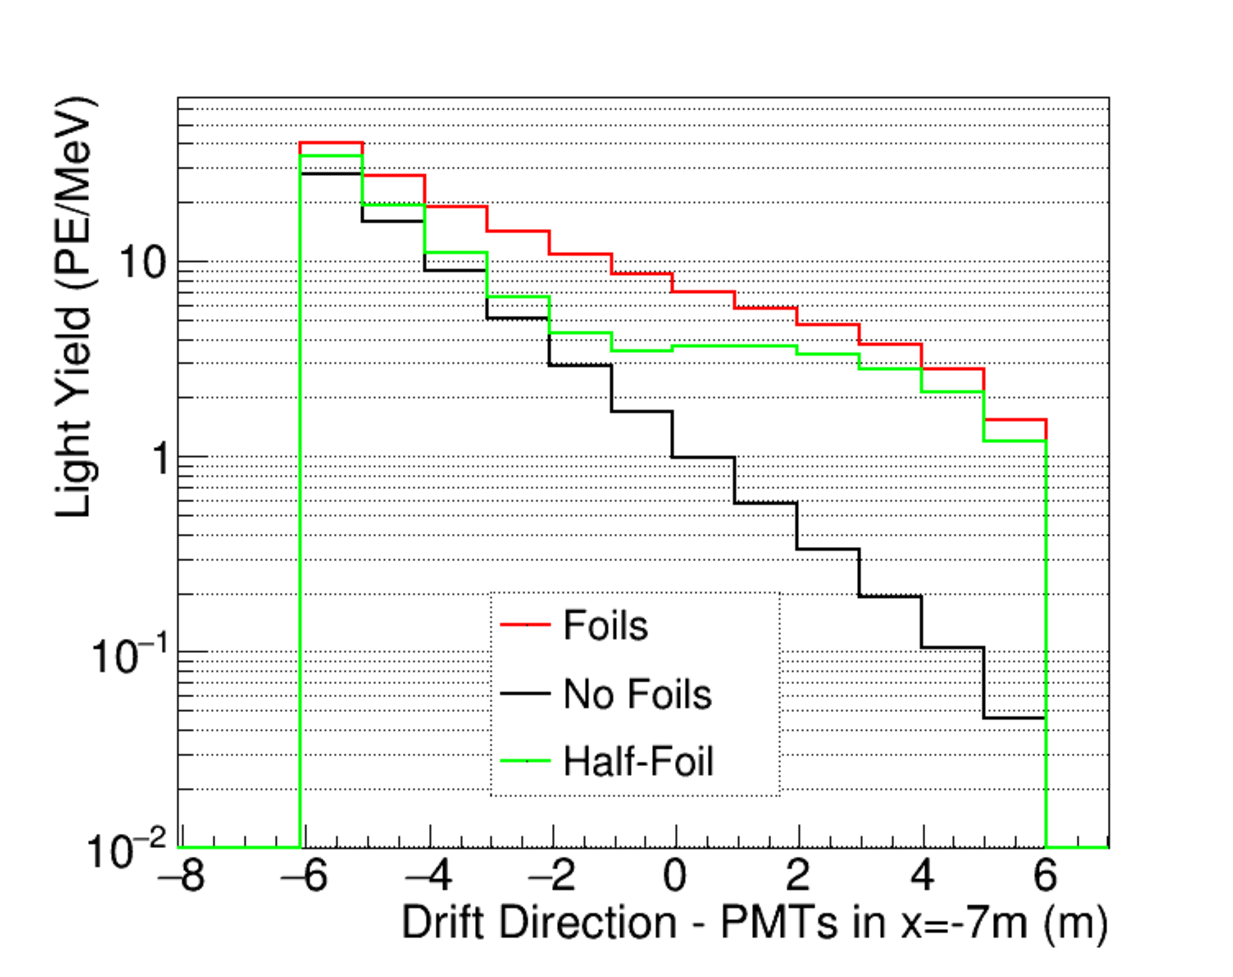
\includegraphics[width=0.49\textwidth]{graphics/dppd_PhotLibProjectionComparison_Drift.pdf}} \hfill
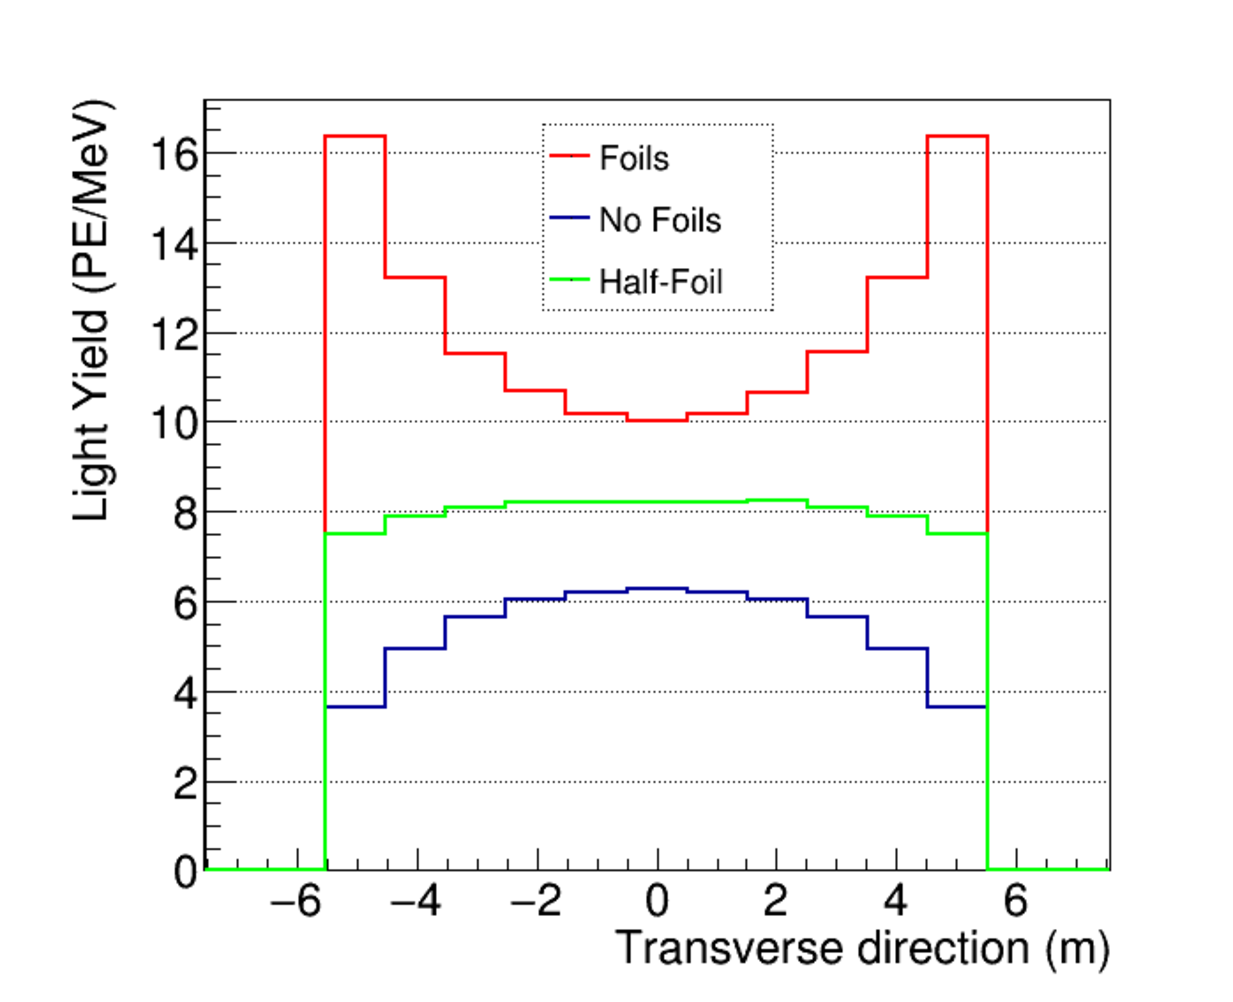
\includegraphics[width=0.49\textwidth]{graphics/dppd_PhotLibProjectionComparison_Trans.pdf}
\end{dunefigure}
 

Figure~\ref{fig:dppd_fd_light_yield} shows the detected light yield, for the half foils baseline geometry, as a function of drift and transverse directions simultaneously, averaged over the beam direction. Near the cathode plane ($Y=$\SI{-6}{m} in this figure) the highest light yield is expected near the center of the active volume ($X=0$). The opposite is true near the anode plane ($Y=$\SI{+6}{m}).  

\begin{dunefigure}[Expected \twod light yield in the full \dshort{dpmod}]{fig:dppd_fd_light_yield}
{Expected light yield in the full \dword{dp} \dword{fd} cryostat, for the half \dword{wls} reflector foils geometry. The yield units are number of photo-electrons per \si{\MeV} of deposited energy. The 2D yield is shown as a function of the drift (vertical axis) and transverse (horizontal axis) directions, averaging over the third spatial coordinate (not shown). The red and blue contours indicate the \dword{tpc} active volume snd the reflective foils position, respectively. The \dwords{pmt} are located at a drift coordinate of \SI{-7}{\m}.}
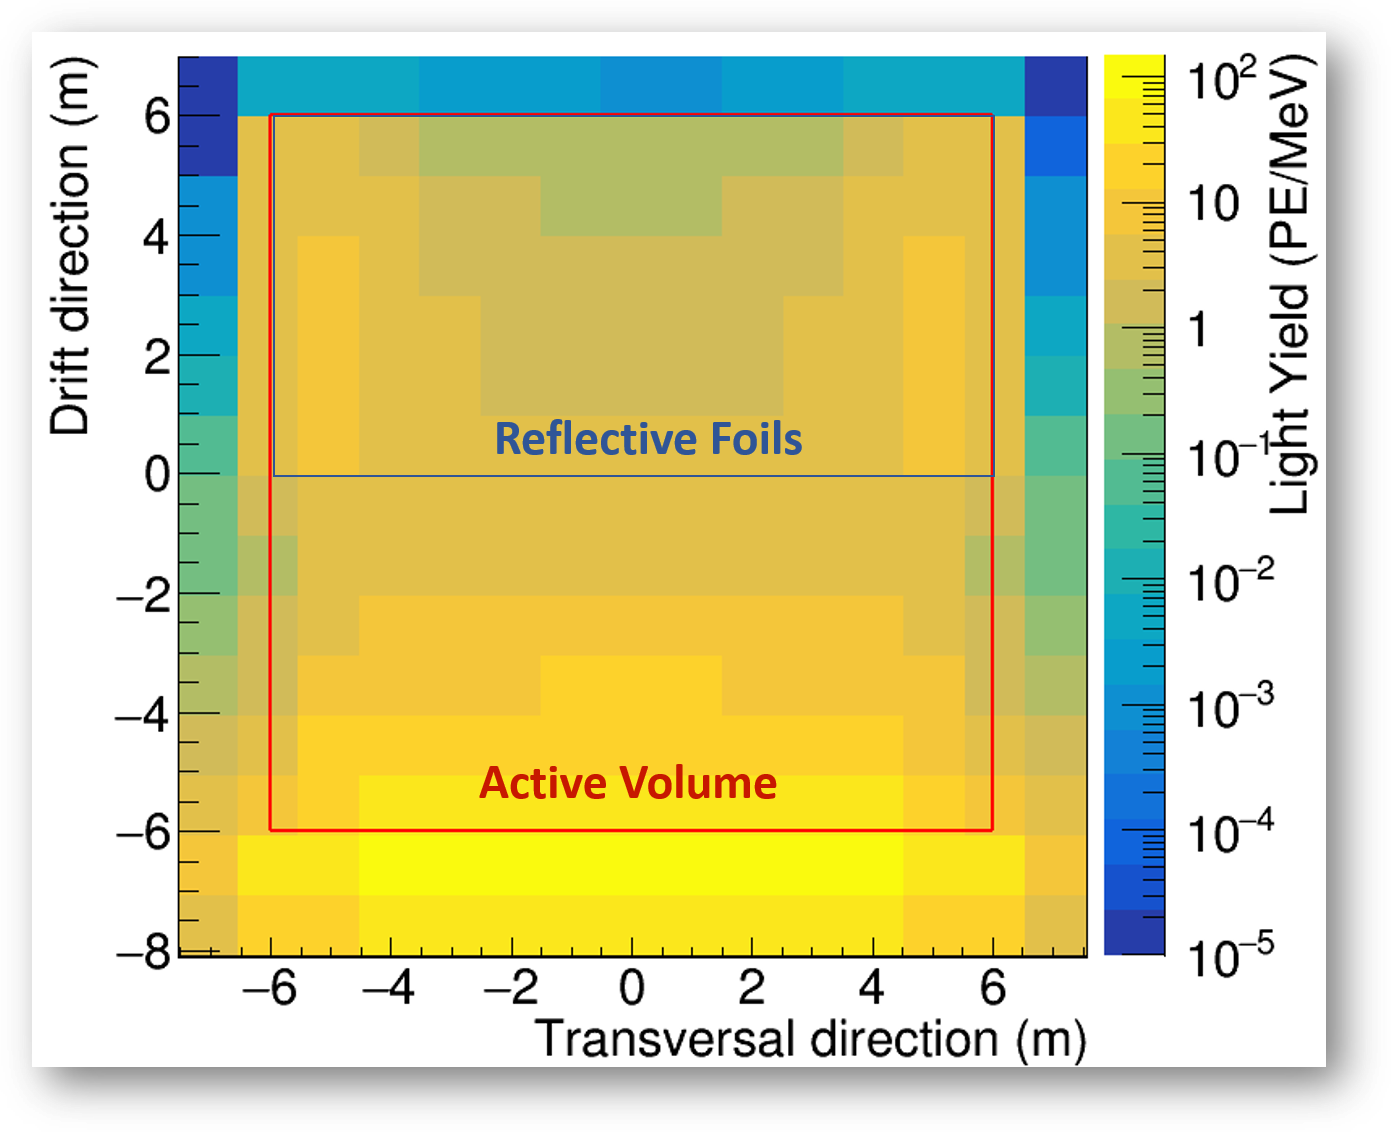
\includegraphics[width=0.65\textwidth]{graphics/dppd_PhotLibHalfFoil.png} 
\end{dunefigure}
